\documentclass[UTF8,b5paper]{ctexart}
\usepackage{geometry}
\usepackage{amsmath}
\usepackage{amsfonts}
\usepackage{float}
\usepackage{amssymb}
\usepackage{graphicx}
\usepackage{subfigure}

\newcommand{\dpm}[1]{$\displaystyle{#1}$}

\geometry{left=1.5cm,right=1.5cm,top=1.5cm,bottom=1.5cm}
\setCJKmainfont{思源宋体 CN}
\setCJKsansfont{更纱黑体 SC}
\setCJKfamilyfont{zhkai}{华文楷体}
\setCJKfamilyfont{zhsong}{思源宋体 CN}
\setCJKfamilyfont{zhhei}{更纱黑体 SC}

\linespread{1.5}
\title{测量电源电动势与内阻}
\author{\textsc{Margatroid}}
\date{2019年2月11日}
\begin{document}
\maketitle
\section{实验原理}
\begin{figure}[H]
  \centering
  \subfigure[原理]{
    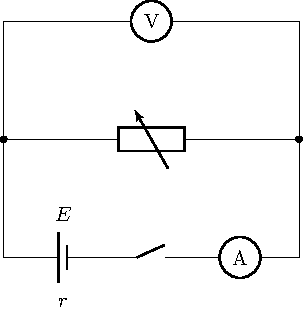
\includegraphics{figs/fig1}
  }
  \subfigure[图象]{
    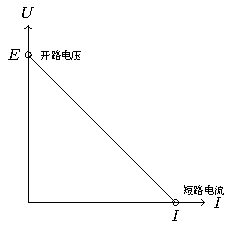
\includegraphics[scale=1.5]{figs/fig2}
  }
  \caption{实验原理}
\end{figure}
如图,通过调节滑动变阻器,可得$U-I$图象如图。则纵轴截距即为开路电压,即电源电动势
,横轴截距为短路电流,斜率的绝对值即为电源内阻。
\section{误差分析}
考虑到电表并不完美,即实际的电流表相当于理想电流表\textbf{串联}一个电阻$R_A$,实际的电压表相当于理想电压表\textbf{并联}一个电阻$R_V$。因此,用该法测出的数值实际上是虚线框内的等效电源的电动势与内阻。

下面分别讨论电流表\textbf{相对电源}内接,外接时的误差情况。
\subsection{电流表内接}
\begin{figure}[H]
  \centering
  \subfigure[原理]{
    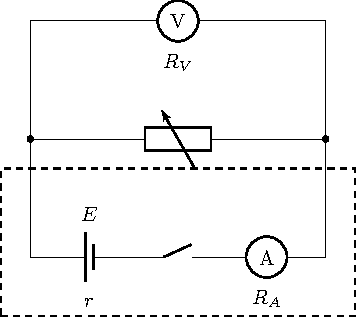
\includegraphics{figs/fig3}
  }
  \subfigure[图象]{
    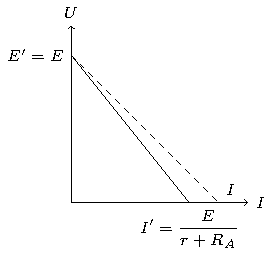
\includegraphics[scale=1.5]{figs/fig4}
  }
  \caption{电流表相对电源内接}
\end{figure}
接下来只需研究虚线框内的电路即可。为了研究其电源电动势$E'$,即开路电压,可将电路「打断」。打断后,电路中无电流,故电流表$R_A$上分得的电压为$0$,因此等效电源的电动势$E'=E$。

考虑等效电源的短路电流,即将等效电源两头短接,显然\dpm{I'=\frac E {r + R_A}}。

考虑等效电源的内阻,显然,我们可以通过\dpm{r' = \frac E {I'} = r + R_A}计算出内阻。不过我们可以尝试另一种方法。即只考虑等效电源内的电阻,然后计算出其阻值大小。对于此图,只考虑等效电源内的电阻时,电路即为$r$与$R_A$串联,因此测得的内阻为$r' = r + R_A$,画出的$U-I$图象如图所示。
\subsection{电流表外接}
\begin{figure}[H]
  \centering
  \subfigure[原理]{
    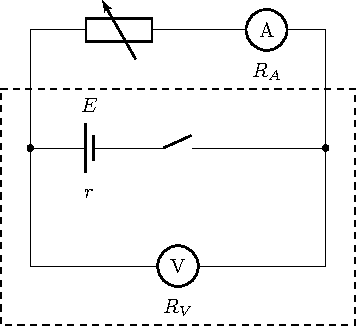
\includegraphics{figs/fig5}
  }
  \subfigure[图象]{
    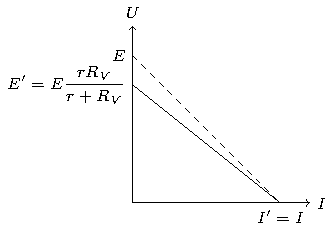
\includegraphics[scale=1.5]{figs/fig6}
  }
  \caption{电流表相对电源外接}
\end{figure}
研究虚线框内的等效电源。首先将电路打断,研究其开路电压,即电动势。打断后,电路变成电源与电压表的串联,故开路电压即电源两端的电压,即路端电压$U$,故\dpm{E'=U=E \frac{R_V}{R_V+r}}。

考虑等效电源的短路电流。将等效电源两侧短路,此时$R_V$被短路,故短路电流\dpm{I'=\frac E r}。

考虑等效电源的内阻,在只考虑等效电源内的电阻时,内电路等价与$r$与$R_V$的并联电路,故\dpm{r'=\frac{rR_V}{r + R_V}},不妨验证一下,\dpm{r'=\frac{E'}{I'} = \frac{rR_V}{r + R_V}}。作$U-I$图象如图所示。
\section{参考}
\begin{itemize}
  \item 维基百科编者。戴维南定理 [G/OL]. 维基百科,2019 (20190211)[2019-02-11].


\end{itemize}
\end{document}
